\documentclass[12pt, twoside]{report_bachelorarbeit}

\usepackage[utf8]{inputenc}
%\input{chapters/Illustrations_preamble}
%\usepackage{pdfpages}

% Images
\usepackage{graphicx}
\usepackage{svg}
\graphicspath{{images/}}
\usepackage[center]{caption} %for captions
\captionsetup{font=small,skip=0pt}
%\usepackage{pgfplots}
%\pgfplotsset{compat=1.17}
\usepackage{tikz} % for generating drawings for NN visualization
\usetikzlibrary{shapes.geometric, positioning}
\usepackage{tikz}
\usepackage{pgfplots}
\pgfplotsset{compat=1.17}
\usetikzlibrary{positioning, shapes.multipart, arrows.meta, calc}

% Comments for Text
\usepackage{xcolor}
\newcommand\TS[1]{\textcolor{red}{[\textbf{WIP}:\emph{#1}]}}

%\usepackage{adjustbox} %rotate environemnts like figures or tables
%\usepackage{makecell} %line break in tables
%\usepackage{pgf}


% Visualizing Algorithms
%\usepackage{algorithm}
%\usepackage{algpseudocode}

% PaperLayout
\usepackage[a4paper, margin=25mm]{geometry}

% For Titlepage
\usepackage{subcaption}
\usepackage{caption}

% Font
\usepackage{newtxtext,newtxmath}
\usepackage{setspace}
\usepackage[absolute]{textpos} % needed for titlepage

%% Header/Footer
\usepackage{lastpage} 
\usepackage{fancyhdr} %Fooder und Header Style

\fancypagestyle{plain}{
	\fancyhf{}
	\fancyhead{}
	\fancyhead[RO,LE]{\centering Computer Vision Seminar: Surgical-Dino}
	\fancyfoot{}
	\fancyfoot[LE,RO]{\thepage}
	%\fancyfoot[LO,CE]{Chapter \thechapter}
	%\fancyfoot[LO,CE]{\ifnum\value{chapter}>0Chapter \thechapter\fi}
	\fancyfoot[CO,RE]{Tilman Seeßelberg}
	\renewcommand{\headrulewidth}{0.4pt}% Line at the header invisible
	\renewcommand{\footrulewidth}{0.4pt}% Line at the footer visible
}
\pagestyle{fancy}
\setlength{\headheight}{14.5pt}
\fancyhead{}
\fancyhead[RO,LE]{\centering \centering Computer Vision Seminar: Surgical-Dino}
\fancyfoot{}
\fancyfoot[LE,RO]{\thepage}
\fancyfoot[LO,CE]{Chapter \thechapter}
%\fancyfoot[LO,CE]{\ifnum\value{chapter}>0\thechapter\fi} 
\fancyfoot[CO,RE]{Tilman Seeßelberg}
\renewcommand{\headrulewidth}{0.4pt}
\renewcommand{\footrulewidth}{0.4pt}

% Hyperlinks
\usepackage{hyperref}
\hypersetup{
	%bookmarks=true,                     % show bookmarks bar
	unicode=false,                      % non - Latin characters in Acrobat’s bookmarks
	pdftoolbar=false,                        % show Acrobat’s toolbar
	pdfmenubar=false,                        % show Acrobat’s menu
	pdffitwindow=false,                 % window fit to page when opened
	pdfstartview={FitH},                    % fits the width of the page to the window
	pdftitle={\centering Computer Vision Seminar: Surgical-Dino},% title
	pdfauthor={Tilman Seeßelberg},                 % author
	pdfsubject={Computer Vision Seminar},                   % subject of the document
	pdfcreator={Tilman Seeßelberg},                   % creator of the document
	pdfproducer={Tilman Seeßelberg},             % producer of the document
	pdfkeywords={NDT, thesis, cfrp, opencv},   % list of keywords
	pdfnewwindow=true,                  % links in new window
	colorlinks=true,                        % false: boxed links; true: colored links
	linkcolor=blue,                          % color of internal links
	linkbordercolor= {0 0 1},
	filecolor=blue,                     % color of file links
	citecolor=blue,                     % color of file links
	urlcolor=blue,                        % color of external links
	menubordercolor= {1 0 0}	
} 
%\providecommand*\algorithmautorefname{Algorithm} %autoref fix to print Algorithm X when ref-ing
%\def\subsectionautorefname{Subsection}
%\def\sectionautorefname{Section}

%Language
\usepackage[USenglish,american]{babel}

%Literaturverzeichniss
\usepackage[style=ieee, backend=biber, dashed=false, doi=true, isbn=true, url=true, eprint=false]{biblatex} 
\addbibresource{./sources.bib}
%\setcounter{biburllcpenalty}{7000} %Line Break for long URLs in bibliography
%\setcounter{biburlucpenalty}{8000} % Line Break for long URLs in bibliography
\usepackage{csquotes} % needed to display quotes according to language

% Acronyms
\usepackage[nohyperlinks]{acronym}

% Mathematics packages
\usepackage{siunitx}

% List environment
\usepackage{enumitem}

% suppressing errormassages
\hbadness = 10000
\clubpenalty = 10000
\widowpenalty = 10000
\displaywidowpenalty = 10000

%Defining new format commands
\newcommand{\tecterm}[1]{\emph{#1}}

%Syntax Highlighting
%\usepackage{minted}
\usepackage{listings} % include code from file in appendix
\usepackage{xcolor} % for color in code
\definecolor{codegreen}{rgb}{0,0.6,0}
\definecolor{codegray}{rgb}{0.5,0.5,0.5}
\definecolor{codepurple}{rgb}{0.58,0,0.82}
\definecolor{backcolour}{rgb}{0.95,0.95,0.92}
\lstdefinestyle{mystyle}{
    backgroundcolor=\color{backcolour},   
    commentstyle=\color{codegreen},
    keywordstyle=\color{magenta},
    numberstyle=\tiny\color{codegray},
    stringstyle=\color{codepurple},
    basicstyle=\ttfamily\footnotesize,
    breakatwhitespace=false,         
    breaklines=true,                 
    captionpos=b,                    
    keepspaces=true,                 
    numbers=left,                    
    numbersep=5pt,                  
    showspaces=false,                
    showstringspaces=false,
    showtabs=false,                  
    tabsize=2
}
\lstset{style=mystyle}

%End Plugins
%%%%%%%%%%%%%%%%%%%%%%%%%%%%%%%%%%%%%%%%%%%%%%%%

\begin{document}
\pagestyle{plain}

\begin{titlepage} % Suppresses displaying the page number on the title page and the subsequent page counts as page 1
	\newcommand{\HRule}{\rule{\linewidth}{0.5mm}} % Defines a new command for horizontal lines, change thickness here
	
	\center % Centre everything on the page
	
	%------------------------------------------------
	%	Headings
	%------------------------------------------------
	
	\textsc{\LARGE Darmstadt University of Applied Sciences}\\[1.5cm] % Main heading such as the name of your university/college
	
	\textsc{\Large Computer Vision Seminar}\\[0.5cm] % Major heading such as course name
	
	%\textsc{\large Minor Heading}\\[0.5cm] % Minor heading such as course title
	
	%------------------------------------------------
	%	Title
	%------------------------------------------------
	
	\HRule\\[0.4cm]
	
	{\huge\bfseries Unearthing Surgical-Dino}\\[0.4cm] % Title of your document
	
	\HRule\\[1.5cm]
	
	%------------------------------------------------
	%	Author(s)
	%------------------------------------------------

	\begin{flushleft}
		\large
		\textit{Author}\\
		Tilman \textsc{Seeßelberg} % Your name
	\end{flushleft}

	\begin{flushleft}
		\large
		\textit{Reviewer}\\
		Prof. Dr. Andreas \textsc{Weinmann}, Darmstadt University of Applied Sciences\\
        Vladyslav \textsc{Polushko}, Darmstadt University of Applied Sciences\\
	\end{flushleft}	
%	\begin{flushleft}
%		\large
%		\textit{Supervisors}\\
%		Prof. Dr. Edmond \textsc{Cretu}, University of British Columbia\\ % Supervisor's name
%		Prof. Dr. Robert \textsc{Rohling}, University of British Columbia\\
%		M.Sc. Jonas \textsc{Welsch}, University of British Columbia\\
%		M.Eng. Dominik \textsc{Görick}, German Aerospace Center
%		
%	\end{flushleft}

%\begin{textblock*}{0.3\textwidth}(0.15\textwidth,26cm)
%\begin{minipage}[b]{0.3\textwidth}
%	\includegraphics[height=2cm]{logo_hm}
%\end{minipage}
%\end{textblock*}
%
%\begin{textblock*}{0.3\textwidth}(0.55\textwidth,26cm)
%\begin{minipage}[b]{0.3\textwidth}
%	\includegraphics[height=2cm]{logo_ubc}
%\end{minipage}
%\end{textblock*}
%\begin{textblock*}{0.3\textwidth}(0.75\textwidth,26cm)
%\begin{minipage}[b]{0.3\textwidth}
%	\includegraphics[height=2cm]{logo_dlr}
%\end{minipage}
%	\end{textblock*}

%\begin{figure}[!b]
%\minipage{0.33\textwidth}
%	\includegraphics[width=0.33\linewidth]{logo_hm}
%\endminipage\hfill
%\minipage{0.33\textwidth}
%	\includegraphics[width=0.33\linewidth]{logo_dlr}
%\endminipage\hfill
%\minipage{0.33\textwidth}
%	\includegraphics[width=0.33\linewidth]{logo_ubc}
%\endminipage
%\end{figure}

\begin{figure}[!b]

\centering
%\includegraphics[width=.3\textwidth]{logo_hm}\hfill
\includesvg[width=.8\textwidth]{images/h_da.svg}\hfill
%\includegraphics[width=.3\textwidth]{logo_dlr}
\end{figure}

	% If you don't want a supervisor, uncomment the two lines below and comment the code above
	%{\large\textit{Author}}\\
	%John \textsc{Smith} % Your name
	
	%------------------------------------------------
	%	Date
	%------------------------------------------------
	
	\vfill\vfill\vfill % Position the date 3/4 down the remaining page
	
	{Date of Submission: \large\today} % Date, change the \today to a set date if you want to be precise
	
	%------------------------------------------------
	%	Logo
	%------------------------------------------------
	
	%\vfill\vfill
	%\includegraphics[width=0.2\textwidth]{placeholder.jpg}\\[1cm] % Include a department/university logo - this will require the graphicx package
	 
	%----------------------------------------------------------------------------------------
	
	\vfill % Push the date up 1/4 of the remaining page
	
\end{titlepage}

\pagenumbering{roman}
\section*{Abstract}
\addcontentsline{toc}{chapter}{Abstract}
\input{chapters/00_abstract}
\newpage
\section*{Kurzzusammenfassung}
\addcontentsline{toc}{chapter}{Kurzzusammenfassung}
\input{chapters/00_kurzzusammenfassung}
\newpage
%\subsection*{Preamble}
%\addcontentsline{toc}{chapter}{Preamble}
%\input{chapters/preamble}


\tableofcontents
\listoffigures
\listoftables

% create acronyms
\chapter*{List of abbreviations}
\begin{acronym}
\acro{mlp}[MLP]{Multi Layer Perceptron}
\end{acronym}

\pagestyle{fancy}
\setlength{\headheight}{14.5pt}
\fancyhead{}
\fancyhead[RO,LE]{\centering Computer Vision Seminar: Surgical-Dino}
\fancyfoot{}
\fancyfoot[LE,RO]{\thepage}
\fancyfoot[LO,CE]{Chapter \thechapter}
%\fancyfoot[LO,CE]{\ifnum\value{chapter}>0\thechapter\fi} 
\fancyfoot[CO,RE]{Tilman Seeßelberg}
\renewcommand{\headrulewidth}{0.4pt}
\renewcommand{\footrulewidth}{0.4pt}

\chapter{Introduction}
\pagenumbering{arabic}
\setcounter{page}{1}
% This report will dive into the findings of the paper \emph{Surgical-DINO: adapter learning of foundation models for depth estimation in endoscopic surgery} by Cui et al.~\cite{Cui2024}.
% The paper introduces a fine tuning regiment for a computer vision foundation model called DINOv2 created by Oquab et al.~\cite{Oquab2023} for the task of Monocular Depth Estimation (MDE) in endoscopy using comparably small dataset of $17607$ frames including a corresponding ground truth depth map.
% This work illustrates the potential of foundation models to accelerate the development of new state of the art models even in domains with limited data availability.
% Foundation models gain more and more tracktion in the field of computer vision as a lot of effort is put into developing unsupervised pretraining tasks for large scale models such as Vision Transformers (ViTs) or other architectures like Convolutional Neural Networks (CNNs).
% Foundation models at the moment seem to be very promising of being the new standard of machine learning models in the field of computer vision, where one would not start from training a network from scratch but rather use a pretrained model and only fine-tune it as it potentionally provides way better results while consuming a lot less computational ressources due to the benefits of the model already having learned meaningful patterns for the data it was trained on.
% An additional advantage is, that it is also possible to achieve good results only using very few labeled data to fine-tune a foundation model.
% Therefor this is also very promissing in the field of medicine, where there are many very expensive prodecures for creating MRI images or similar, or also in endoscopy, where depth maps are needed in order to percicly move the endoscope inside the patient.

\TS{Rewrite and get to the topic (Surgical Dino) quicker}
Foundation models are gaining significant traction in the field of computer vision, driven by extensive research in unsupervised pretraining tasks for large-scale models such as Vision Transformers (ViTs) and Convolutional Neural Networks (CNNs). 
These models promise to become the new standard in machine learning for computer vision, offering substantial advantages over training networks from scratch. 
By leveraging pretrained models and fine-tuning them, researchers can achieve impressive results, often surpassing previous state-of-the-art performance while reducing computational resources and the need of large labled datasets, due to the foundation models already having learned meaningful representations of the input data.
This is particularly advantageous in the medical field. 
In disciplines like endoscopy, where creating labeled datasets is expensive and time-consuming, foundation models offer a promising solution.
For instance, in endoscopy, accurate depth maps are crucial for precisely navigating the endoscope within the patient. 
By fine-tuning a pretrained foundation model, significant advancements can be made compared to training from scratch.

This report delves into the findings of the paper \emph{Surgical-DINO: Adapter Learning of Foundation Models for Depth Estimation in Endoscopic Surgery} by Cui et al.~\cite{Cui2024}. 
The paper introduces a fine-tuning regimen for a computer vision foundation model, DINOv2, developed by Oquab et al.~\cite{Oquab2023}, specifically tailored for the task of Monocular Depth Estimation (MDE) in endoscopy. 
Using the comparatively small dataset SCARED dataset~\cite{Allan2021} with $17\,607$ unique images, each accompanied by a corresponding ground truth depth map, this work highlights the potential of foundation models to accelerate the development of state-of-the-art techniques, even in domains with limited data availability.

This report will first dive into Vision Transformer (ViTs) in Section~ref{sec:vision-transformers}, followed by a detailed explanation of the used foundation model DINOv2 in Section~\ref{sec:dino} after which the basics of depth estimation are layed out in Section~\ref{sec:depth-estimation} before the details of fine-tuning foundation models are explained in Section~\ref{sec:model-fine-tuning} before.
\TS{polish the last sentence}
\chapter{Theoretical Foundations}
\section{Vision Transformer}\label{sec:vision-transformer}
Vision Transformers (ViTs), as introduced by Dosovitskiy et al. in 2020~\cite{Dosovitskiy2020}, build on the work of Vaswani et al.~\cite{Vaswani2017}, adapting the transformer architecture for image classification. 
ViTs leverage the transformer's strengths in handling sequential data by splitting an image into a sequence of $16\times16$ pixel patches and processing them through the transformer architecture just like tokens as explained below.
\begin{figure}[h]
    \centering
    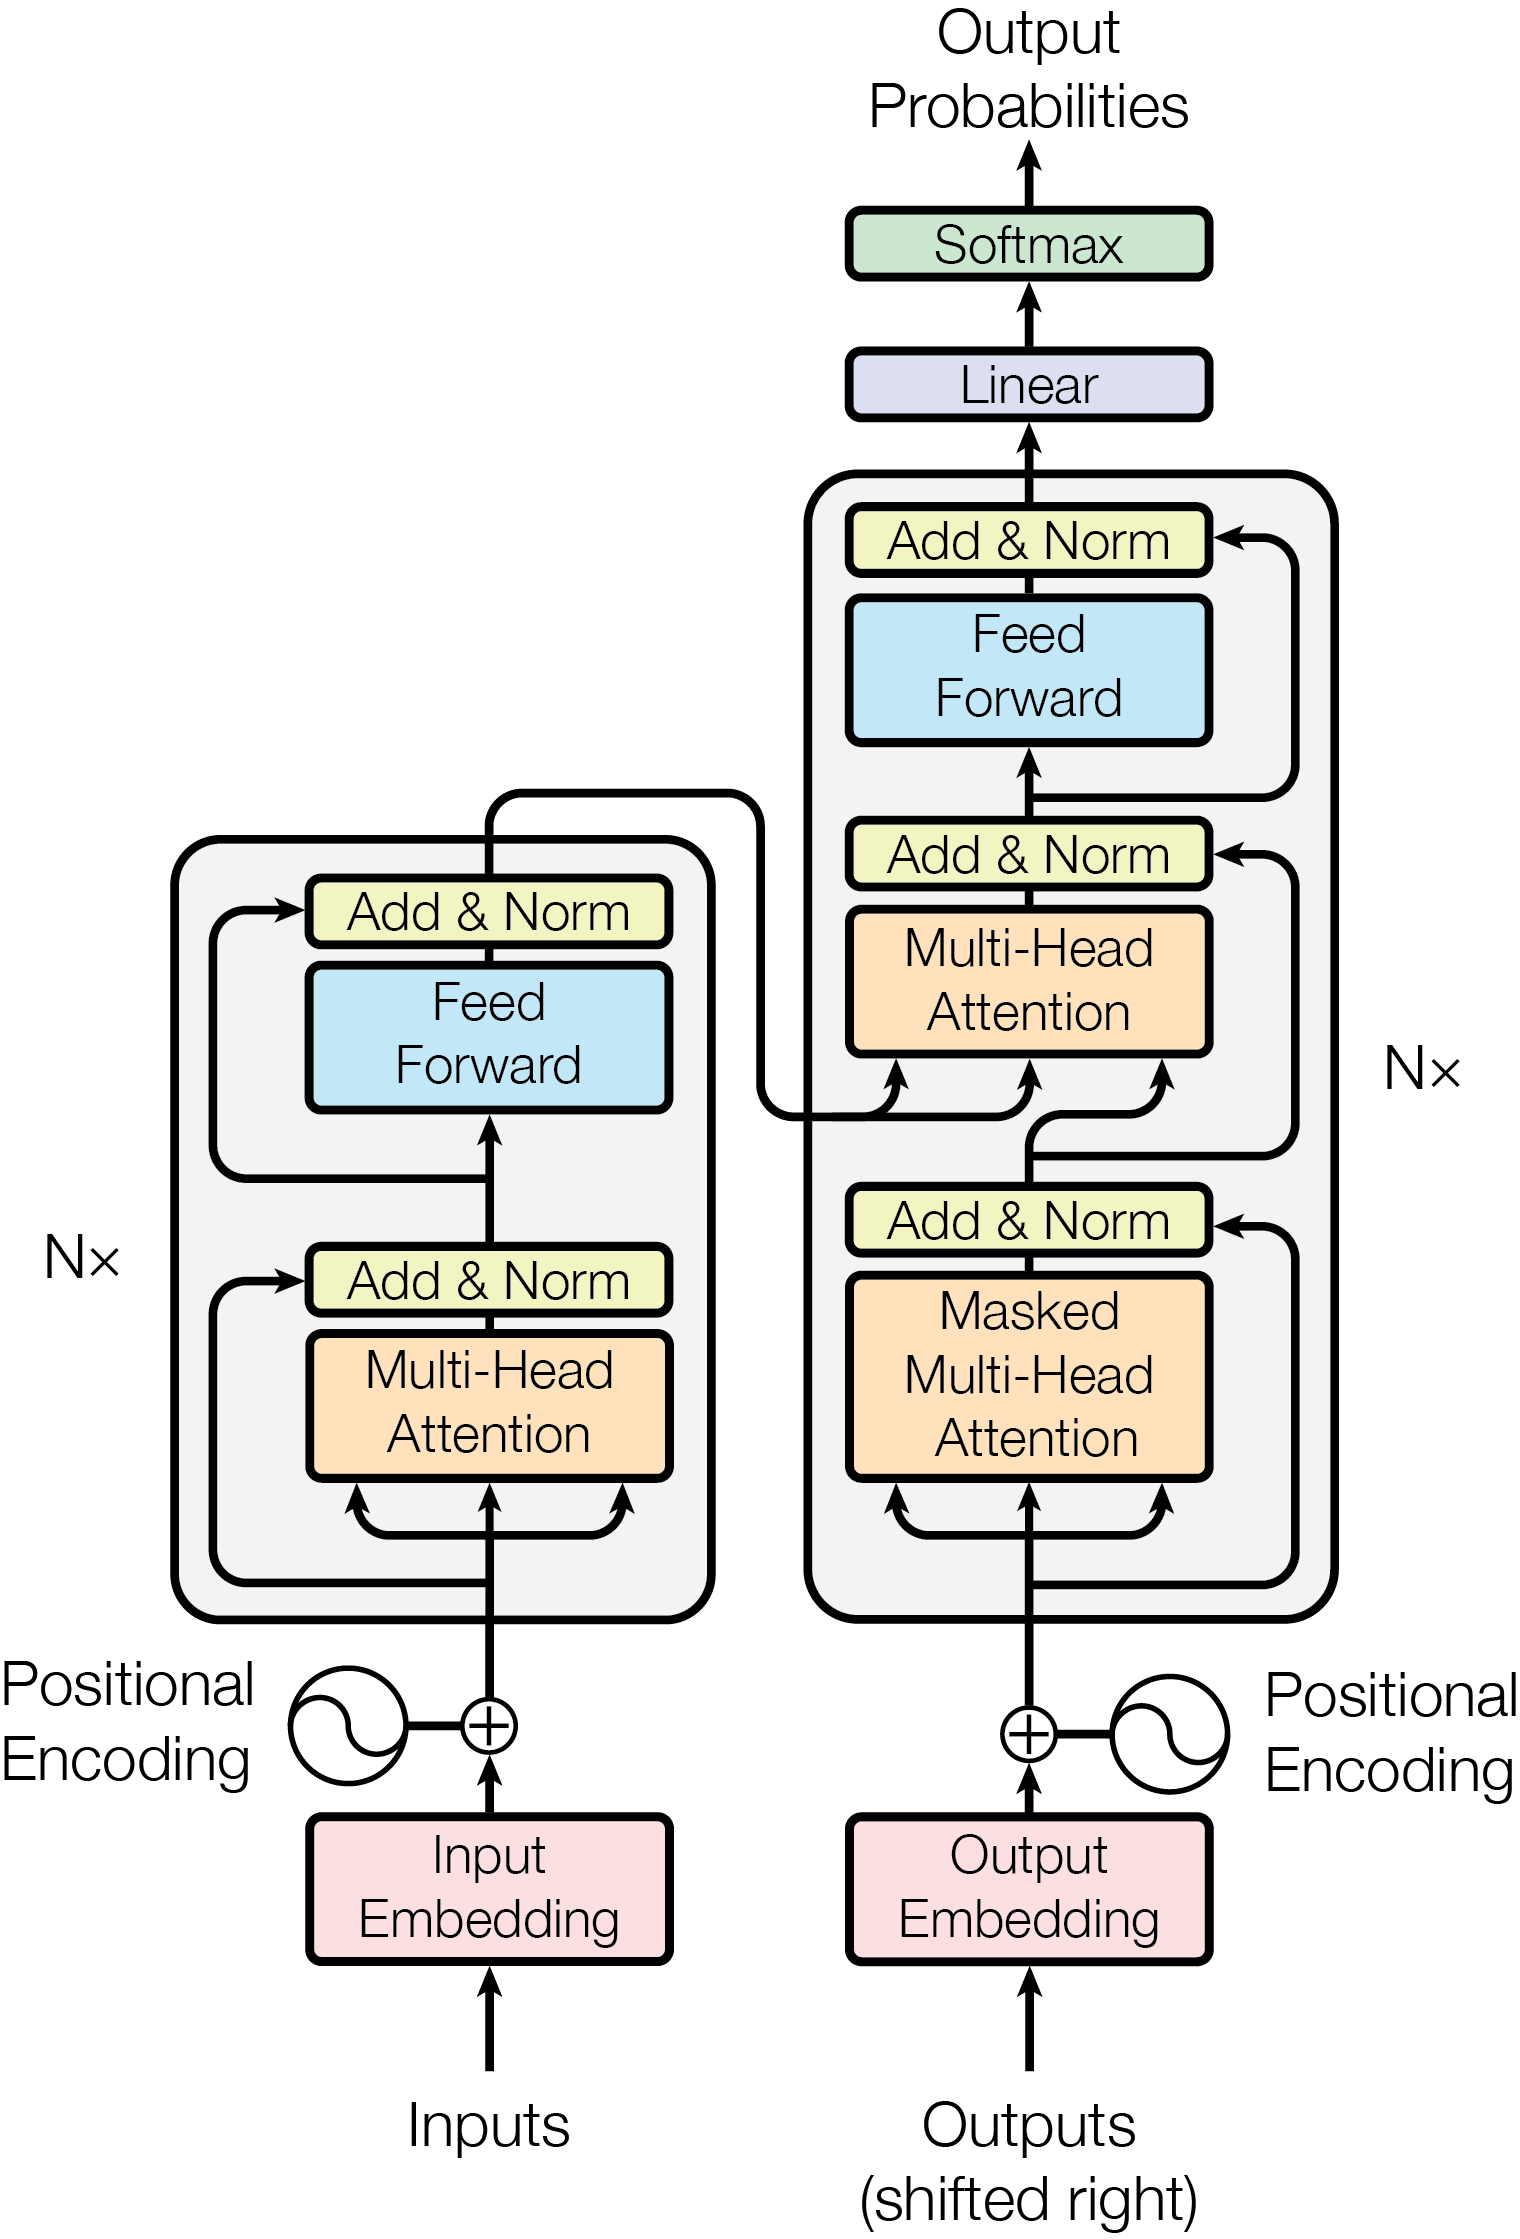
\includegraphics[width=0.3\textwidth]{images/TransformerArchitectureVaswani2017TransformerPage3.png}
    \caption[The original transformer architecture]{The transformer architecture (image from~\cite{Vaswani2017})}\label{fig:transformer}
\end{figure}

The original transformer architecture, designed for machine translation, consists of an encoder-decoder structure that processes input sequences through \emph{embedding layers}, \emph{positional encoding}, \emph{attention mechanisms}, and \emph{multi-layer perceptrons}. 
The following describes these components in the context of the original transformer architecture which is illustrated in Figure~\ref{fig:transformer}.

\textbf{Embedding Layer:} To ingest a sequence into a transformer, it is first split into smaller pieces called tokens, which can be words, subwords, or characters, and are then mapped into continuous vector representations called \emph{token vectors}. 
These \emph{token vectors} form the \emph{Embedding Matrix}.

\textbf{Positional Encoding:} Following the embedding a \emph{positional encoding matrix} is added to the \emph{Embedding Matrix}, which gives the model a hint of the order of the tokens in the sequence. 
This is needed as Transformers do not have an inductive bias about token order, unlike predecessors like Recurrent Neural Networks (RNNs)~\cite{Salehinejad2018} or Long Short-Term Memory (LSTM) networks~\cite{Hochreiter1997}.

\textbf{Encoder:} Next, the \emph{Embedding Matrix} is processed by a \emph{Multi-Head Attention} consisting of $h$ \emph{Attention Heads}.
The original paper achieved good results with $h=8$.
An Attention head first runs the \emph{Embedding Matrix} through three learnable linear layers $W^Q, W^K \&\, W^V$ in parallel, producing three matrices: \emph{query matrix} $Q$, \emph{key matrix} $K$, and \emph{value matrix} $V$ each $\in \mathrm{R}^{d_{\text{model}\times d_k}}$ with $d_{\text{model}}$ being the length of a token vector (512 in the original paper) and $d_k = \frac{d_{\text{model}}}{h}$. 
These terms are analogous to database operations, where the query matrix is the search query, the key matrix is the database, and the value matrix is the data in the database. 
These terms try to convey the intuition behind the attention mechanism.
These matrices are processed by one or more \emph{Attention Heads} as shown in Equation~\ref{eq:attention} to calculate the attention score using the Scaled Dot-Product Attention method. 
First the query matrix $Q$ and the transposed key matrix $K$ is multiplied, devided by the square of the dimension of the matrices $d_k$ and then normalized using softmax to prevent exploding gradients.
This dot product is the \emph{Attention Matrix} of dimension $d_{\text{model}}\times d_{\text{model}}$ which contains the \emph{Attention Scores} which can be interpreted as probabilities of how much a certain token is correlated to another token \textbf{Explained in a good manner here~\cite{Han2023}}. 
This \emph{Attention Matrix} then multiplied with the value matrix $V$ resulting in the weighted value matrix.
Having $h$ attention heads leads to $h$ weighted value matrices which are concatenated and processed by a final linear layer $W^O \in \mathrm{R}^{hd_k \times d_{\text{model}}}$.
\begin{equation}
    \text{Attention}(Q, K, V) = \text{softmax}\left(\frac{QK^{T}}{\sqrt{d_{k}}}\right)V
    \label{eq:attention}
\end{equation}
Following the multi-headed attention mechanism, the resulting 

\textbf{Decoder:} The original Transformer architecture includes an encoder-decoder structure, where the encoder processes the input sequence and the decoder generates the output sequence token by token. While both encoder and decoder consist of the same building blocks, the decoder uses a masked multi-headed attention mechanism, zeroing out the lower left triangle of the attention matrix containing the attention scores to prevent the model from attending to future tokens. 
Following that a multi-head cross attention was applied connecting the output of the encoder with the decoder.
Since then works such as the BERT framework by Devlin et al.~\cite{Devlin2018} have shown that the decoder is not inherently needed for tasks like language translation, or text generation allowing for a simplified \emph{Encoder Transformer} architecture.

This methodology is largely copied by the ViT architecture, though slightly adapted as shown in Table~\ref{tab:transformer_vit_comparison}.

\begin{table}[h!]
    \centering
    \begin{tabular}{|p{3cm}|p{5.5cm}|p{5.5cm}|}
    \hline
    \textbf{Component} & \textbf{Transformers} & \textbf{Vision Transformers (ViTs)} \\ \hline
    Embedding & Devides input sequence (e.g., a sentence) into tokens (e.g., syllables) and converts them into continuous vector representations, forming the Embedding Matrix. & Devides the input image into non-overlapping patches of size $16 \times 16$. Each patch is flattened and used as an embedding vector. All embedding vectors together form the Embedding Matrix.\\ \hline
    Position Embedding & Uses fixed 1-d sinusoidal positional encodings to encode the position of each token in the sequence.& Uses learnable position embeddings to better capture the spatial relationships between image patches.\\ \hline
    Encoder & Consists of a stack of identical layers, each with a multi-head self-attention mechanism and a position-wise fully connected feed-forward network. & Same as in Transformers.\\ \hline
    Decoder & Consists of a stack of identical layers, each with a multi-head self-attention mechanism and an multi-head cross attention connecting the output of the encoder with the decoder. The cross attention is followed by a position-wise fully connected feed-forward network. & Not applicable, as ViTs only use an encoder.\\ \hline
    Attention Mechanism & Computes attention scores using query (Q), key (K), and value (V) matrices. Multi-head attention allows the model to attend to different parts of the input sequence simultaneously. &Same as Transformer.\\ \hline
    Class Token & Not applicable. & Introduces a special class token appended to the sequence of patch embeddings, used for classification tasks by aggregating information from all patches.\\ \hline
    \end{tabular}
    \caption{Comparison of Components in Transformers and Vision Transformers}\label{tab:transformer_vit_comparison}
\end{table}

Using this simplified Transformer architecture, as visualized in Figure~\ref{fig:vit}, ViTs have demonstrated superior performance over state-of-the-art convolutional neural networks (CNNs) in several image classification tasks~\cite{Mauricio2023}. 
Since the original ViT paper, many more use cases beyond image classification have emerged for Transformers in the computer vision field, including anomaly detection, object/instance detection and segmentation, image compression and upscaling, dense/depth estimation~\cite{Ranftl2021}, and video image generation~\cite{Jamil2023}. 
Despite requiring significantly more training data than previous state-of-the-art CNN architectures, ViTs effectively leverage the transformer architecture to surpass the previous state of the art, highlighting the importance of unsupervised pre-training on large datasets and the flexibility of transformers in processing different types of data beyond natural language.
\begin{figure}
    \centering
    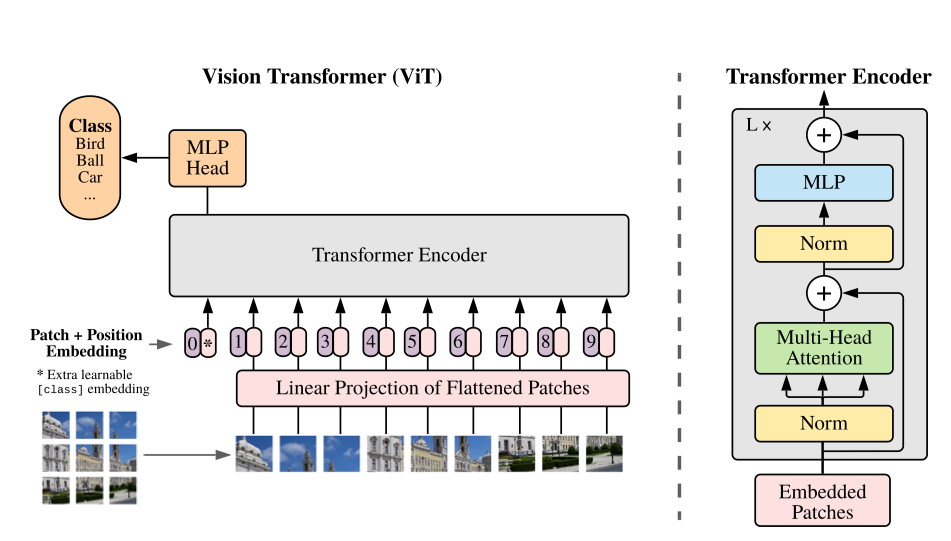
\includegraphics[width=0.8\textwidth]{images/vit_overview.png}
    \caption[The Vision Transformer architecture]{The Vision Transformer architecture (copied from~\cite{Dosovitskiy2020}).}\label{fig:vit}
\end{figure}

\section{Dino and DinoV2}
As mentioned in the privious Section~\ref{sec:vision-transformer}, ViTs are work very well for tasks like image classification and have shown superior performance over state-of-the-art convolutional neural networks (CNNs) in several image classification tasks.
So far ViTs were mostly trained in a supervised manner and needed a lot of labeled data to achieve state-of-the-art performance.
As labeled training data is expensive and time consuming to generate, it is very desirable to train models in an unsupervised manner.
Just a year after the introduction of the Vision Transformer, Caron et al.~\cite{Caron2021} introduced an approach to achieve exactly this called DINO (DIstilled NOt labeled), which is a framework for training in theory any network capable of ingesting image data using self-distillation without labels.
However the paper in particular emphasizes the synergy of Dino with Vision Transformers as a good compromise between performance and computational cost.
Dino is a usefull framework for tasks such as segmentation, depth estimation, and object detection, as it provides a good initialization for supervised fine-tuning.


As explained in~\cite{Phuong2019} destillation in machine learning is a method facilitating the transfer of knowledge from one model to another using a teacher-student model approach.
Often the teacher is a larger complex pretrained model which is used to train a much smaller stundent model. 
However, in the case of Dino the teacher is a non-pretrained model being trained in parallel with the student model. 
This process is called self-distillation, as no pretrained model is used to inject prexisting knowledge into the student model.

In a teacher stundent architecture the student tries to predict the output of the teacher model.
In Dino the students weights get updated using the classical gradient decend approach, while the teacher model is updated using a exponential moving average of the student model weights.
Caron et al. figured that in order to prevent a trivial solution where both teacher and student would start outputing the same output no regard to the input, it is enough to center the output of the teacher model to a mean of 0 and to apply a sharpened softmax function to the output by applying a temperatur parameter $\tau$ called temperatur to the softmax function as shown in equation~\ref{eq:sharp_softmax}. It makes very large values even larger and very small values even smaller.

\textbf{Architecture}

Dino is trained using a classical student teacher network approach, though the teacher is not a pretrained model but a model trained in parallel to the student model.
The Tracher model is largely the same as the student model, but the outputs follow a normalisation applying centering subtracting the mean and running the resulting outputs thorugh a shapened softmax function as shown in equation~\ref{eq:sharp_softmax}.

\begin{equation}
q_{i} = \frac{f_{i}}{|f_{i}|_{2}} \cdot \tau
\label{eq:sharp_softmax}
\end{equation}



- Attention Map right after training puts much attention on the main object of the image and less on the background. This already is a good start for segmentation
- Dino is trained unsupervised and places, when trained, images in to a latent vector, where similar images are close to each other, similar to how similar words are embedded close to each other when training a embedding on them. This could already be used for a k-nearest neighbor approach to classify images.
\subsection{Depth Estimation}
\subsection{Segmentation}

\section{Model Fine-Tuning}
Foundation Models (FMs), as defined in~\cite{Bommasani2021}, are models trained on a large variety of data using self-supervised learning sometimes even for weeks on hunderds of graphic processing units (GPUs) as e.g. the GPT3 model~\cite{Yuan2022} or the Florence CV Foundation Model by Yuan et al.~\cite{Yuan2021}.
These FMs can then fine-tuned doing few shot training, to tailor the FM to a specific task using several magnitutes less data as would be needed for training a model from scratch.
This saves a lot of computational cost and time as it often is enough to retrain only small parts of the FM, and most of the parameters/weights get frozen as well as that cost can be saved dataset which can be relativley small.
Mathematically, the straight forward way of fine-tuning a model is by retraining all parameters, which can be written as in equation~\ref{eq:finetuning} with $W_0$ being the pretrained weights and $\delta W$ the change in weights during fine-tuning.
\begin{equation}
    W' = W_0 + \delta W
    \label{eq:finetuning}
\end{equation}
This However still is relativley computationally intesive as the backpropagation has to be done for all parameters.
\textbf{DISCUSS IN GENERALL HOW PRETRAINING WORKS???}

A more efficient way of fine-tuning weight matrices is Low Rank Adaption (LoRA) as suggested by Hu et al.~\cite{Hu2021} in the context of transformer fine-tuning.
Hut et al. assume based on the the work of Aghajanyan et al.~\cite{Aghajanyan2020}, that the updated weight matrices $\delta W_n$ inside the attention heads of the transformer have a rank much lower then their dimensionality.
In order to utilize this assumption to more efficiently fine-tune a transformer the updated weight matrices $\delta W_n$ are decomposed into two matrices $A \in \mathbb{R}^{d \times r}$ and $B \in \mathbb{R}^{r \times k}$ with $r << d$ and $r << k$ as shown in equation~\ref{eq:lora}.
Hu et al. set the goal to use a maximum of 18M parameters for fine tuning the 173B parameter GPT3 model and created a grid search for optimizing the rank $r$ and which weight matrices to update.
Eventually they figured for their usecase a rank $r = 4$ and only applying updates to all key matrices $K$ and value matrices $V$ in the attention heads of the transformer performed the best.
Besides the advantage of significantly lowering the computational cost of only optimizing the $A$ and $B$ matrices, fine-tuning using LoRa does not increase inference times as the decomposed matrices are recomposed and added onto the original weight matrices $W_0$ after the fine tuning and therefor do not add any additional computation to the forward pass of the model.
\begin{equation}
    W = W_0 + BA
    \label{eq:lora}
\end{equation}

\begin{figure}
    \centering
    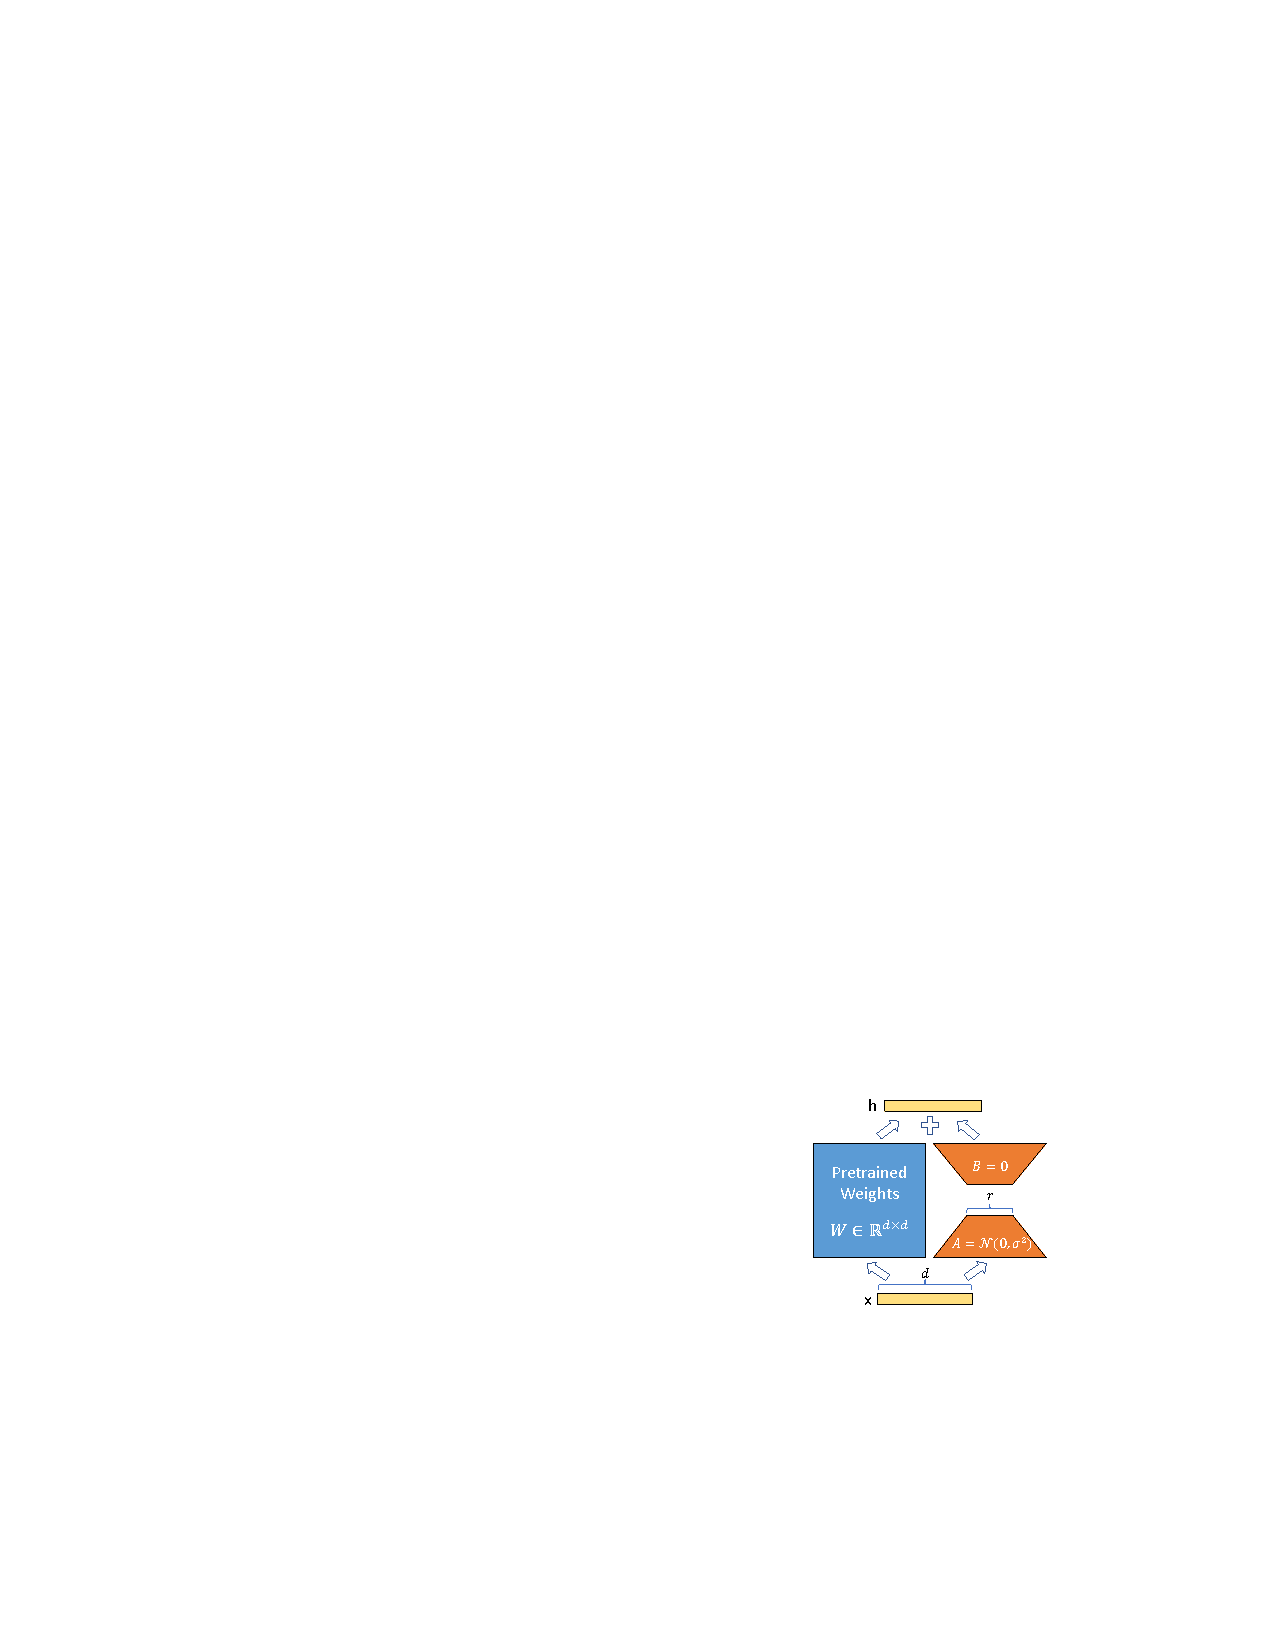
\includegraphics[width=0.5\textwidth]{images/Hu2021_LoraArch.pdf}
    \caption{LoRa architecture with the docomposed $\delta W_n = AB$ and their initialization  method (graphic lifted from~\cite{Hu2021})}\label{fig:loraarch}
\end{figure}

Another methodology of finetuning Neural Networks (NN) is to 
\chapter{Unearthing Surgical-Dino}
\section{Surgical-Dino}

\subsection*{Motivation}
\TS{Information about the motivation of Dino}
Surgical Dino as introduced by Cui et al.~\cite{Cui2024} addresses the challange of monocular depth estimation in endoscopy using a fine-tuned version of the DinoV2 ViT foundation model, which is one of the biggest foundation models available to the public.
Most current works using foundation models in the surgical domain deal with segmentation and object detection tasks.
There, however, is also a need for using foundation models for accurate depth estimation as it is a crucial step to improve technologies in the field of robotic surgery and has the potential of enhacing 3d reconstruction of interal organs and surgical navigation.
While there are endoscopy instruments available using stereo cameras for depth estimation, these are only available on the most advanced surgical robots such as the Davinci Xi, which are not available in most hospitals.
Hence the desire to create appropriate depth estimations using only a singel image using ML algorithms such as CNNs and more recently transformer.
While vision foundation models could already proof their value in more natural domains where there are large datasets available, but the authors of Surgical-Dino figured that the unadapted foundation models experience a significant drop in performance when applied to the surgical domain, which makes sense as this kind of data usually is not inculded in the training data of the foundation models as it often is confidential and not availbale at the scale needed for training such models from scratch.
DinoV2 was choosen as the basis of Surgical-Dino by the authors as it was the most recent foundation model available and already achieved promising results in several computer vision tasks including depth estimation in more general settings such as autonomous driving or general segmentation.

\subsection*{Implementation}
\TS{Information about the technicalities of the model}
To adapt DinoV2, which was introduced in~\ref{fig:dinov1}, for depth estimation in the surgical domain the authors develope a pipeline to finetune the smallest of the available pretrained DinoV2 Encoders called \emph{DINOv2-S} with 12 transformer blocks and a token vector size of $d_{\text{model}}=784$ each block containing multi-head attention blocks with 6 heads and additionally add a new depth prediction head to transfer the Transformer Block outputs, also known as \emph{Embedding Matrix} or \emph{Feature Map} into a grayscale depth map with pixel values between $0$ to $255$.
For the finetuning all weights of the \emph{DINOv2-S} model were frozen and extented by adding trainable LoRa side layers as introduced in Section~\ref{sec:model-fine-tuning} to all Attention Heads' query and value matrices inspired by the findings of Zhang et al.~\cite{Zhang2021}. 
Using LoRa side layers was decided on by the authors as they allow to fine tune the model with very limited computational ressources and small datasets, do not increase the inference time later on and are easy to implement. 
In case of this work a single highend consumer grade graphics card was enough to train the model in a reasonable amount of time.

Following the transformer encoder blocks a depth decoder head is appended which converts not only the \emph{Feature Maps} of the last transformer block, but the outputs of every third block. 
Before the decoder head the \emph{Feature Maps}  are unflattend 

Following the transformer encoder blocks a depth decoder head is appended which converts not only the \emph{Feature Maps} of the last transformer block, but the outputs of every third block. 
Before the decoder head, each \emph{token vector} of inside the \emph{Feature Maps} gets unflattened and upsampled to $f\times$ the original patch resolution using bilinear interpolation to increase the resolution of the depth map.
These transformed features are then concatenated along the channel dimension to form Each Feature Matrix then is reassambled and the different Features Maps are concatenated along the channel dimension.
Finally, the depth decoder utilizes a $1\times1$ convolutional layer to predict the depth of each pixel individually, treating depth prediction as a classification problem by dividing the depth range into discrete bins.

% The depth map the authors decided to treat this problem as a pixel classification problem and add a single convolutional layer following the transformer blocks to predict the depth of each pixel.

First the outputs not just of the last transformer block but also of the transformer blocks 3, 6 and 9 are processed by the depth prediction head.
Before that the transformer block outputs are unflattend, to have the same shape as the input patches, bi-linearly upsampled 4x to increase the resolution for the depth map. At the end the Depth map is downsampled again which improves the overall quality of the depth map.


\subsection*{Training}
\TS{Results of the Paper}

The first step for creating Surgical-DINO is to fine-tune the DinoV2 Encoder following the DinoV2 pre-training procedure except with the encoder weights frozen

\textbf{Related Works}

\textbf{Reasoning of the authors for how they derive at the fine-tuning regiment as they do}


\chapter{Discussion}
\TS{Discussing the Results in context of related works}
% \chapter{Conclusion}
% \input{chapters/06_conclusion}
\addcontentsline{toc}{chapter}{Bibliography}
\clearpage
\pagestyle{plain}
\printbibliography

\appendix
\chapter{Architecture Comparison Transformer and Vision Transformer}\label{app:CompViT}

\begin{table}[h!]
    \centering
    \begin{tabular}{|p{3cm}|p{5.5cm}|p{5.5cm}|}
    \hline
    \textbf{Component} & \textbf{Transformers} & \textbf{Vision Transformers (ViTs)} \\ \hline
    Embedding & Devides input sequence (e.g., a sentence) into tokens (e.g., syllables) and converts them into continuous vector representations, forming the embedding matrix. & Devides the input image into non-overlapping patches of size $16 \times 16$. Each patch is flattened and used as an embedding vector. All embedding vectors together form the embedding matrix.\\ \hline
    Position Encoding & Uses fixed 1-d sinusoidal positional encodings to encode the position of each token in the sequence.& Uses learnable position embeddings to better capture the spatial relationships between image patches.\\ \hline
    Encoder & \multicolumn{2}{p{11cm}|}{Consists of a stack of identical layers, each with a multi-head self-attention mechanism and a position-wise MLP.}\\ \hline
    Decoder & Consists of a stack of identical layers, each with a multi-head self-attention mechanism and an multi-head cross attention connecting the output of the encoder with the decoder. The cross attention is followed by a position-wise MLP. & Not applicable, as ViTs only use an encoder.\\ \hline
    Attention Mechanism & \multicolumn{2}{p{11cm}|}{Computes attention scores using query (Q), key (K), and value~(V) matrices. Multi-head attention allows the model to attend to different parts of the input sequence simultaneously.}\\ \hline
    Class Token & Not applicable. & Prepends a special class token to the embedding matrix which the prediction head uses for classification\\ \hline
    \end{tabular}
    \caption[Comparison of ViT and Transformer Architecture]{Comparison of Components in the original Transformers by Vaswani et al.~\cite{Vaswani2017} and the original ViT by Dosovitskiy et al.~\cite{Dosovitskiy2020}, detailing key adaptations such as the use of image patches instead of textual tokens and positional embeddings tailored for spatial data, which allow ViTs to effectively handle visual contexts.}
\end{table}


\newpage
%\input{chapters/eidesstattlicherErklärung}
\end{document}